\documentclass[
  12pt,
  oneside,
  a4paper,
  brazil
]{abntex2}

\usepackage[utf8]{inputenc}
\usepackage[T1]{fontenc}
\usepackage{lmodern}
\usepackage{microtype}
\usepackage{graphicx}
\usepackage{float}
\usepackage{amsmath,amssymb}
\usepackage{booktabs}
\usepackage{siunitx}
\usepackage{tikz}
\usepackage{indentfirst}
\usepackage{hyperref}
\usepackage{abntex2cite}
\usetikzlibrary{arrows.meta,positioning,shapes.geometric}

\sisetup{
  output-decimal-marker = {,},
  per-mode = symbol
}

\hypersetup{
  colorlinks=true,
  linkcolor=black,
  citecolor=black,
  urlcolor=black,
  pdfauthor={Seu Nome},
  pdftitle={Plataforma Didática Embarcada para Reprodução de Arquivos COMTRADE e Emulação de Relés de Proteção}
}

\setlength{\parindent}{1.25cm}
\setlength{\parskip}{0.2cm}

% Estilo dos títulos de capítulo no formato:
% "Capítulo 1" em uma linha e o título do capítulo abaixo.
\makechapterstyle{capitulo-tcc}{%
  \renewcommand{\chapnamefont}{\normalfont\huge\bfseries}
  \renewcommand{\chapnumfont}{\normalfont\huge\bfseries}
  \renewcommand{\chaptitlefont}{\normalfont\Huge\bfseries}
  \renewcommand{\printchaptername}{\chapnamefont\chaptername}
  \renewcommand{\printchapternum}{\chapnumfont\space\thechapter}
  \renewcommand{\afterchapternum}{\par\vspace{1.6\onelineskip}}
  \renewcommand{\printchaptertitle}[1]{\chaptitlefont ##1}
  \setlength{\beforechapskip}{0pt}
  \setlength{\afterchapskip}{2.5\onelineskip}
}

\chapterstyle{capitulo-tcc}

\titulo{Plataforma Didática Embarcada para Reprodução de Arquivos COMTRADE e Emulação de Relés de Proteção em Sistemas Elétricos de Potência}
\autor{Seu Nome}
\local{Manaus-AM}
\data{2026}
\orientador{Prof. Dr. Nome do Orientador}
\instituicao{%
  Universidade Federal do Amazonas
  \par
  Faculdade de Tecnologia
  \par
  Engenharia Elétrica - Eletrotécnica}
\tipotrabalho{Monografia}
\preambulo{Monografia apresentada à Coordenação do Curso de Engenharia Elétrica - Eletrotécnica da Universidade Federal do Amazonas, como parte dos requisitos necessários à obtenção do título de Engenheiro Eletricista.}

\begin{document}

\imprimircapa
\imprimirfolhaderosto

\begin{dedicatoria}
  \vspace*{\fill}
  \begin{flushright}
    Dedico este trabalho aos meus familiares, professores e colegas que contribuíram para minha formação acadêmica e profissional.
  \end{flushright}
\end{dedicatoria}

\begin{agradecimentos}
Agradeço primeiramente a Deus, à minha família, ao meu orientador e aos professores que contribuíram para minha formação. Agradeço também aos colegas que acompanharam o desenvolvimento deste trabalho e contribuíram com discussões, testes e sugestões ao longo do projeto.
\end{agradecimentos}

\begin{epigrafe}
  \vspace*{\fill}
  \begin{flushright}
    ``A teoria sem a prática vira verbalismo, assim como a prática sem teoria vira ativismo.''

    Paulo Freire
  \end{flushright}
\end{epigrafe}

\begin{resumo}
Este trabalho apresenta o desenvolvimento de uma plataforma didática embarcada para reprodução de arquivos COMTRADE e emulação de funções de proteção aplicadas a sistemas elétricos de potência. A proposta utiliza duas placas ESP32: uma responsável pela geração de sinais analógicos de tensão e corrente, a partir de oscilografias simuladas, e outra responsável pela recepção das amostras e execução dos algoritmos de proteção. As oscilografias são obtidas por meio de simulações de faltas trifásicas no Simulink, convertidas para o padrão COMTRADE e posteriormente processadas para reprodução física por meio de um conversor digital-analógico MCP4728. No sistema receptor, os sinais são amostrados, tratados e utilizados na avaliação de funções de proteção, como sobrecorrente, direcional e distância. A plataforma busca aproximar o ensino teórico de proteção de sistemas elétricos de potência de uma experiência prática, acessível e reconfigurável, permitindo aos estudantes observar a relação entre sinais de falta, processamento fasorial e atuação de relés digitais.

\vspace{\onelineskip}

\noindent
\textbf{Palavras-chave}: COMTRADE; ESP32; relés de proteção; sistemas elétricos de potência; plataforma didática; proteção digital.
\end{resumo}

\begin{resumo}[Abstract]
\begin{otherlanguage*}{english}
This work presents the development of an embedded educational platform for COMTRADE file playback and emulation of protection functions applied to electric power systems. The proposed platform uses two ESP32 boards: one responsible for generating analog voltage and current signals from simulated oscillographic records, and another responsible for receiving the samples and executing protection algorithms. The oscillographic records are obtained from three-phase fault simulations in Simulink, converted to the COMTRADE standard, and then processed for physical playback through an MCP4728 digital-to-analog converter. In the receiving system, the signals are sampled, processed, and used to evaluate protection functions such as overcurrent, directional, and distance protection. The platform aims to bring the theoretical teaching of power system protection closer to a practical, accessible, and reconfigurable experience, allowing students to observe the relationship between fault signals, phasor processing, and digital relay operation.

\vspace{\onelineskip}

\noindent
\textbf{Keywords}: COMTRADE; ESP32; protection relays; electric power systems; educational platform; digital protection.
\end{otherlanguage*}
\end{resumo}

\pdfbookmark[0]{\listfigurename}{lof}
\listoffigures*
\cleardoublepage

\pdfbookmark[0]{\listtablename}{lot}
\listoftables*
\cleardoublepage

\pdfbookmark[0]{\contentsname}{toc}
\tableofcontents*
\cleardoublepage

\textual

\chapter{Introdução}

Os sistemas elétricos de potência são estruturas fundamentais para o fornecimento de energia elétrica à sociedade moderna, abrangendo as etapas de geração, transmissão, distribuição e consumo. Para que esses sistemas operem de forma segura e confiável, é necessário empregar dispositivos capazes de identificar condições anormais de operação e atuar de maneira adequada para isolar trechos defeituosos. Nesse contexto, os sistemas de proteção exercem papel essencial, pois são responsáveis por detectar faltas, sobrecorrentes, variações de tensão e outras perturbações que possam comprometer a integridade dos equipamentos e a continuidade do fornecimento de energia \cite{anderson1999power,blackburn2006protective}.

Entre os dispositivos utilizados na proteção de sistemas elétricos de potência, destacam-se os relés de proteção. Esses equipamentos recebem sinais de tensão e corrente do sistema, processam essas grandezas e tomam decisões de atuação com base em critérios previamente definidos. Com o avanço da tecnologia digital, os relés passaram a empregar algoritmos de processamento de sinais, estimação fasorial e lógicas de proteção configuráveis, permitindo maior flexibilidade, precisão e integração com sistemas de supervisão e análise de eventos \cite{phadke2009computer,horowitz2014power}.

Apesar da importância desses conceitos para a formação do engenheiro eletricista, o ensino de proteção de sistemas elétricos de potência ainda é, em muitos casos, predominantemente teórico. A formação de futuros engenheiros de proteção demanda contato com fundamentos, ajustes, testes e análise de desempenho de relés, pois a área envolve não apenas conhecimento conceitual, mas também interpretação de eventos e tomada de decisão baseada em sinais reais ou simulados \cite{brahma2009education}. Entretanto, a utilização de equipamentos reais de proteção, malas de teste e simuladores especializados costuma ser limitada em ambientes acadêmicos devido ao custo elevado, à complexidade de operação e à necessidade de infraestrutura laboratorial específica. Como consequência, temas como atuação de relés, análise de oscilografias, ajustes de proteção, estimação de fasores e comportamento dos sinais durante faltas podem permanecer distantes da experiência prática dos estudantes.

Diante dessa limitação, torna-se relevante o desenvolvimento de ferramentas didáticas acessíveis que permitam aproximar os conteúdos teóricos de uma experiência prática em bancada. Na educação em engenharia, atividades laboratoriais e estratégias de aprendizagem ativa são reconhecidas por favorecer a compreensão de fenômenos físicos, o desenvolvimento de habilidades experimentais e a conexão entre teoria e prática \cite{prince2004active,feisel2005laboratory}. No ensino de proteção de sistemas elétricos, plataformas laboratoriais têm sido propostas justamente para permitir que estudantes configurem relés, observem condições de falta e avaliem mecanismos de atuação de forma experimental \cite{ferris2013protectionlab,radhi2020plc}. Nesse contexto, o uso de microcontroladores de baixo custo, como o ESP32, associado a conversores digital-analógicos e a arquivos padronizados de oscilografia, possibilita a construção de uma plataforma experimental capaz de reproduzir sinais de tensão e corrente e avaliar algoritmos de proteção em condições controladas.

Neste trabalho, propõe-se uma plataforma didática embarcada para reprodução de arquivos COMTRADE e emulação de funções de relés de proteção aplicadas a sistemas elétricos de potência. O padrão COMTRADE é amplamente utilizado para armazenamento e intercâmbio de registros oscilográficos, permitindo representar sinais provenientes de simulações ou medições reais \cite{ieee_comtrade,iec_60255_24_2013}. No projeto desenvolvido, as oscilografias são obtidas a partir de simulações de faltas trifásicas realizadas no Simulink, convertidas para arquivos COMTRADE e posteriormente reproduzidas por uma ESP32 geradora com auxílio de um conversor digital-analógico MCP4728 \cite{espressif_esp32,microchip_mcp4728}.

A plataforma é constituída basicamente por duas unidades ESP32. A primeira unidade é responsável pela geração e reprodução dos sinais analógicos de tensão e corrente a partir das amostras provenientes dos arquivos COMTRADE. A segunda unidade realiza a recepção dos sinais reproduzidos, a aquisição das amostras e a execução dos algoritmos de proteção. Nas versões mais recentes do projeto, o sistema passou a ter maior grau de embarcamento, com a comunicação, a reprodução, a recepção e os algoritmos de proteção concentrados nas ESP32, enquanto os scripts em computador atuam principalmente na preparação dos dados, configuração, supervisão e interface de execução.

Do ponto de vista acadêmico, a principal contribuição deste trabalho está na construção de uma plataforma acessível, reconfigurável e orientada ao ensino, capaz de permitir que estudantes observem a relação entre uma falta simulada, a oscilografia correspondente, a reprodução física dos sinais e a resposta dos algoritmos de proteção. Dessa forma, busca-se complementar o ensino teórico de proteção de sistemas elétricos de potência com uma ferramenta prática, de baixo custo e compatível com a realidade de laboratórios didáticos, reforçando a importância de experiências laboratoriais no processo de formação em engenharia \cite{feisel2005laboratory,ferris2013protectionlab}.

\section{Objetivos}

\subsection{Objetivo geral}

Desenvolver uma plataforma didática embarcada, baseada em microcontroladores ESP32, para reprodução de sinais provenientes de arquivos COMTRADE e emulação de funções de relés de proteção aplicadas a sistemas elétricos de potência.

\subsection{Objetivos específicos}

Para alcançar o objetivo geral, foram definidos os seguintes objetivos específicos:

\begin{itemize}
  \item realizar simulações de faltas trifásicas em um sistema elétrico de potência no ambiente Simulink/Matlab;
  \item exportar as amostras de tensão e corrente obtidas nas simulações para o ambiente de processamento do Matlab;
  \item converter as amostras simuladas para o padrão COMTRADE, gerando os arquivos \texttt{.cfg} e \texttt{.dat};
  \item validar os arquivos COMTRADE quanto ao tipo de arquivo, número de canais, taxa de amostragem e compatibilidade com a plataforma desenvolvida;
  \item desenvolver o sistema embarcado de geração dos sinais analógicos de tensão e corrente utilizando ESP32 e conversor digital-analógico MCP4728;
  \item implementar a comunicação entre o computador e a ESP32 geradora para envio, organização e reprodução das amostras;
  \item desenvolver o sistema embarcado de recepção dos sinais analógicos reproduzidos pela unidade geradora;
  \item processar as amostras recebidas para extração de grandezas utilizadas pelos algoritmos de proteção;
  \item implementar funções de proteção, como sobrecorrente, direcional e distância, conforme os recursos disponíveis na plataforma;
  \item permitir a configuração dos algoritmos de proteção por meio de comandos e parâmetros de ajuste, aproximando a operação do sistema da lógica de configuração de relés reais;
  \item avaliar a resposta da plataforma diante das oscilografias de falta reproduzidas;
  \item analisar a aplicabilidade do sistema como ferramenta didática para o ensino de proteção de sistemas elétricos de potência.
\end{itemize}

\section{Organização do trabalho}

Este trabalho está organizado em seis capítulos. O Capítulo 1 apresenta a introdução, contextualizando o tema, a motivação do projeto, a proposta da plataforma desenvolvida e os objetivos do trabalho.

O Capítulo 2 apresenta a fundamentação teórica necessária ao desenvolvimento do projeto, abordando conceitos relacionados a sistemas elétricos de potência, curtos-circuitos, relés de proteção, arquivos COMTRADE e processamento digital de sinais aplicado à proteção.

O Capítulo 3 descreve a metodologia adotada, incluindo a geração das oscilografias no Simulink, a conversão das amostras para o padrão COMTRADE, a validação dos arquivos e a arquitetura geral da plataforma composta pelas unidades de geração e recepção.

O Capítulo 4 apresenta a implementação do sistema, detalhando os principais componentes de hardware e software, os scripts desenvolvidos, os firmwares das ESP32, o protocolo de comunicação, a bufferização das amostras, a reprodução dos sinais e a estrutura dos algoritmos de proteção.

O Capítulo 5 apresenta os resultados e discussões, contemplando a análise dos sinais reproduzidos e recebidos, a resposta das funções de proteção implementadas, as limitações observadas e a aplicabilidade didática da plataforma.

Por fim, o Capítulo 6 apresenta as considerações finais do trabalho, destacando as principais contribuições, as limitações do sistema desenvolvido e sugestões para trabalhos futuros.

\chapter{Conceitos Fundamentais de Sistemas Elétricos de Potência}

Este capítulo apresenta os conceitos fundamentais utilizados no desenvolvimento da plataforma proposta. Inicialmente, são abordadas noções gerais sobre sistemas elétricos de potência, com destaque para as grandezas elétricas utilizadas no projeto. Em seguida, são discutidos os curtos-circuitos em sistemas elétricos, os princípios da proteção, as funções de relés implementadas na plataforma, o padrão COMTRADE e os fundamentos de processamento digital de sinais aplicados a relés digitais.

A fundamentação teórica apresentada neste capítulo tem como objetivo estabelecer a base necessária para compreender a arquitetura do sistema desenvolvido, no qual sinais de tensão e corrente provenientes de simulações são reproduzidos em bancada e utilizados para avaliação de algoritmos de proteção.

\section{Sistemas elétricos de potência}

Um sistema elétrico de potência pode ser entendido como o conjunto de instalações e equipamentos responsáveis pela geração, transmissão, distribuição e utilização da energia elétrica. Em sua estrutura básica, a energia é produzida em unidades geradoras, transportada por linhas de transmissão em níveis elevados de tensão, reduzida em subestações e finalmente entregue aos consumidores por redes de distribuição.

\begin{figure}[H]
  \centering
  \caption{Diagrama unifilar de um sistema elétrico de potência}
  \label{fig:diagrama-sep}
  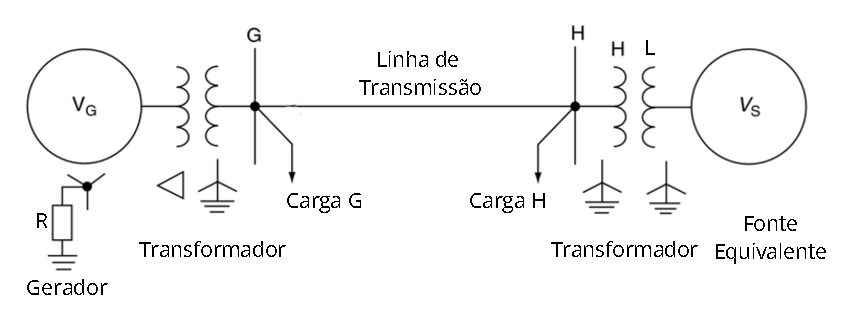
\includegraphics[width=0.94\textwidth]{figuras/sistema_eletrico_potencia_v2_cortado.pdf}
  \legend{Fonte: Adaptado de \citeonline{blackburn2006protective}.}
\end{figure}

A operação desses sistemas exige o equilíbrio contínuo entre geração e carga, além da manutenção de grandezas como tensão, corrente, frequência e potência dentro de limites adequados. Alterações bruscas de carga, falhas em equipamentos, descargas atmosféricas, curtos-circuitos e manobras podem provocar perturbações que afetam a estabilidade, a segurança e a continuidade do fornecimento de energia elétrica \cite{kundur1994power,glover2017power}.

No contexto deste trabalho, as grandezas mais importantes são tensão, corrente, potência, impedância e frequência. Para sinais senoidais em regime permanente, a tensão instantânea pode ser representada por:

\begin{equation}
  v(t) = V_m \sin(\omega t + \theta),
  \label{eq:tensao-instantanea}
\end{equation}

\noindent em que $V_m$ é o valor de pico, $\omega = 2\pi f$ é a frequência angular e $\theta$ é o ângulo de fase. O valor eficaz de uma grandeza senoidal é dado por:

\begin{equation}
  V_{\text{rms}} = \frac{V_m}{\sqrt{2}}.
  \label{eq:vrms}
\end{equation}

Em sistemas trifásicos equilibrados, as potências ativa, reativa e aparente podem ser expressas por:

\begin{align}
  P &= \sqrt{3} V_L I_L \cos\varphi, \label{eq:potencia-ativa}\\
  Q &= \sqrt{3} V_L I_L \sin\varphi, \label{eq:potencia-reativa}\\
  S &= \sqrt{3} V_L I_L, \label{eq:potencia-aparente}
\end{align}

\noindent em que $V_L$ é a tensão de linha, $I_L$ é a corrente de linha e $\varphi$ é o ângulo entre tensão e corrente. A impedância elétrica, por sua vez, pode ser representada por:

\begin{equation}
  Z = R + jX = \frac{\bar{V}}{\bar{I}},
  \label{eq:impedancia}
\end{equation}

\noindent sendo $\bar{V}$ e $\bar{I}$ os fasores de tensão e corrente. Essa relação é particularmente importante para a função de distância, pois a impedância aparente vista pelo relé é calculada a partir dos fasores medidos.

No projeto desenvolvido, os sinais de tensão e corrente são gerados por simulações computacionais, convertidos para COMTRADE e reproduzidos em bancada. Portanto, as equações apresentadas servem de base para a interpretação das amostras reproduzidas e para o cálculo das grandezas utilizadas pelos algoritmos de proteção.

\section{Curtos-circuitos em sistemas elétricos de potência}

O curto-circuito é uma das condições anormais mais relevantes em sistemas elétricos de potência. Ele ocorre quando há uma conexão de baixa impedância entre pontos que deveriam permanecer eletricamente separados. Como consequência, podem surgir correntes elevadas, afundamentos de tensão e esforços térmicos e mecânicos capazes de danificar equipamentos e comprometer a operação do sistema \cite{anderson1999power,blackburn2006protective}.

Os principais tipos de curto-circuito são:

\begin{itemize}
  \item curto-circuito trifásico, envolvendo simultaneamente as três fases;
  \item curto-circuito bifásico, envolvendo duas fases;
  \item curto-circuito bifásico-terra, envolvendo duas fases e a terra;
  \item curto-circuito monofásico-terra, envolvendo uma fase e a terra.
\end{itemize}

As faltas trifásicas são classificadas como simétricas, pois, idealmente, preservam o equilíbrio entre as fases. Já as faltas monofásicas, bifásicas e bifásicas-terra são assimétricas e exigem análise por componentes simétricas. Embora a falta trifásica não seja a mais frequente em sistemas reais, ela é uma das mais severas e é amplamente utilizada em estudos iniciais de curto-circuito e proteção.

\begin{figure}[H]
  \centering
  \caption{Representação simplificada de uma falta trifásica em um sistema elétrico}
  \label{fig:falta-trifasica}
  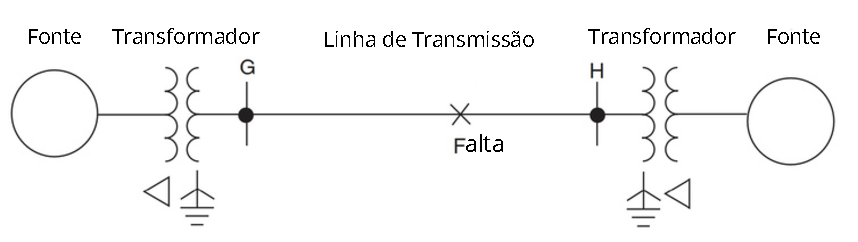
\includegraphics[width=0.92\textwidth]{figuras/SEP_falta_br_cortado.pdf}
  \legend{Fonte: Adaptado de \citeonline{blackburn2006protective}.}
\end{figure}

Para uma falta trifásica, a análise pode ser feita por fase, utilizando o equivalente de Thévenin visto do ponto de falta. A corrente de curto-circuito trifásico é dada por:

\begin{equation}
  I_{cc,3\phi} = \frac{V_{\text{th}}}{Z_{\text{th}} + Z_f},
  \label{eq:icc-trifasico}
\end{equation}

\noindent em que $V_{\text{th}}$ é a tensão de Thévenin por fase, $Z_{\text{th}}$ é a impedância equivalente do sistema até o ponto de falta e $Z_f$ é a impedância da falta. Para uma falta sólida, em que $Z_f \approx 0$, a expressão pode ser aproximada por:

\begin{equation}
  I_{cc,3\phi} \approx \frac{V_{LL}}{\sqrt{3}Z_{\text{th}}},
  \label{eq:icc-solido}
\end{equation}

\noindent sendo $V_{LL}$ a tensão de linha no ponto analisado antes da falta. A potência de curto-circuito trifásica associada pode ser calculada por:

\begin{equation}
  S_{cc,3\phi} = \sqrt{3}V_{LL}I_{cc,3\phi}.
  \label{eq:scc}
\end{equation}

Para faltas assimétricas, as expressões utilizam as impedâncias de sequência positiva, negativa e zero. Por exemplo, para uma falta monofásica-terra, a corrente de falta pode ser expressa por:

\begin{equation}
  I_f = \frac{3V_{\text{fase}}}{Z_1 + Z_2 + Z_0 + 3Z_f}.
  \label{eq:falta-monofasica}
\end{equation}

Neste trabalho, o destaque é dado à falta trifásica, pois ela permite validar a cadeia principal da plataforma com menor complexidade matemática: geração da oscilografia, conversão para COMTRADE, reprodução dos sinais, aquisição pela ESP32 receptora e avaliação das funções de proteção.

\section{Proteção de sistemas elétricos de potência}

A proteção de sistemas elétricos de potência tem como finalidade identificar condições anormais de operação e comandar a isolação seletiva do trecho defeituoso. Para isso, são empregados dispositivos como transformadores de corrente, transformadores de potencial, relés de proteção, disjuntores e sistemas de comunicação e supervisão.

Um sistema de proteção deve atender a critérios fundamentais. A seletividade está relacionada à capacidade de isolar apenas a parte defeituosa do sistema. A sensibilidade indica a capacidade de detectar faltas dentro da zona protegida. A velocidade está associada ao tempo necessário para detectar e eliminar a falta. A confiabilidade envolve a atuação correta quando necessária e a não atuação em situações indevidas \cite{anderson1999power,horowitz2014power}.

Com a evolução dos relés eletromecânicos para relés estáticos e digitais, tornou-se possível implementar múltiplas funções de proteção em um mesmo equipamento. Relés digitais utilizam amostras de sinais de tensão e corrente, realizam processamento numérico e aplicam lógicas configuráveis para determinar se determinada condição exige atuação \cite{phadke2009computer}. Essa característica é explorada neste trabalho por meio da emulação de funções de proteção em uma plataforma embarcada.

\section{Funções de relés de proteção}

As funções de proteção são frequentemente identificadas por números padronizados, conforme a norma IEEE C37.2, que define números e acrônimos para dispositivos e funções utilizados em sistemas elétricos, subestações e instalações de geração \cite{ieee_c37_2_2022}. Essa padronização facilita a documentação técnica, a interpretação de diagramas e a comunicação entre profissionais da área.

No projeto desenvolvido, as funções de relés são tratadas como algoritmos configuráveis. A lógica básica de decisão pode ser representada por uma comparação entre a grandeza medida, extraída das amostras, e um valor de ajuste definido pelo usuário. Em geral, a atuação pode ser expressa por:

\begin{equation}
  \text{atuação} =
  \begin{cases}
    1, & \text{se a condição de atuação permanece verdadeira por } t \geq T_{\text{ajuste}},\\
    0, & \text{caso contrário}.
  \end{cases}
  \label{eq:trip-generico}
\end{equation}

\noindent A seguir, são descritas as principais funções consideradas no contexto da plataforma.

\subsection{Relé de subtensão}

O relé de subtensão, identificado pelo número ANSI 27, atua quando a tensão medida permanece abaixo de um valor previamente ajustado. Essa função é utilizada para detectar afundamentos de tensão, perda de alimentação, falhas em barras, problemas de excitação em máquinas ou condições que possam prejudicar a operação adequada de cargas e equipamentos.

Uma forma usual de parametrização é definir o ajuste em valor por unidade:

\begin{equation}
  V_{pu} = \frac{V_{\text{medido}}}{V_{\text{nominal}}}.
  \label{eq:vpu}
\end{equation}

\noindent Em uma proteção com dois estágios, as condições podem ser representadas por:

\begin{equation}
  V_{pu} \leq V_{27,i}\quad\text{(instantânea)},\qquad
  V_{pu} \leq V_{27,t}\ \text{por}\ t\geq T_{27}\quad\text{(temporizada)}.
  \label{eq:subtensao}
\end{equation}

O estágio temporizado responde a uma subtensão moderada persistente, enquanto o estágio instantâneo é reservado a uma tensão remanescente mais baixa e, portanto, mais crítica. O \textit{pickup} é identificado assim que um ciclo fasorial válido cruza o limiar; a temporização condiciona o \textit{trip}, não a detecção da condição.

\subsection{Relé de sobretensão}

O relé de sobretensão, identificado pelo número ANSI 59, atua quando a tensão medida excede um valor de ajuste. Essa função é aplicada na proteção de equipamentos contra elevações anormais de tensão, que podem ocorrer em rejeição de carga, manobras, falhas de regulação ou sobretensões temporárias.

Utilizando a mesma representação em por unidade da Equação \ref{eq:vpu}, os dois estágios podem ser expressos por:

\begin{equation}
  V_{pu} \geq V_{59,i}\quad\text{(instantânea)},\qquad
  V_{pu} \geq V_{59,t}\ \text{por}\ t\geq T_{59}\quad\text{(temporizada)}.
  \label{eq:sobretensao}
\end{equation}

O estágio temporizado responde a uma elevação moderada e persistente, enquanto o estágio instantâneo atua diante de uma sobretensão mais severa. Em uma plataforma didática, essa separação permite comparar a influência conjunta da magnitude e do tempo sobre a decisão do relé.

\subsection{Relé de sobrecorrente}

O relé de sobrecorrente é uma das funções mais utilizadas em sistemas de proteção. Ele atua quando a corrente medida ultrapassa um valor de \textit{pickup} previamente definido. De acordo com a aplicação, pode assumir forma instantânea, associada ao número ANSI 50, ou temporizada, associada ao número ANSI 51 \cite{blackburn2006protective,ieee_c37_2_2022}.

A condição de atuação instantânea pode ser representada por:

\begin{equation}
  I_{\text{medido}} \geq I_{50,\text{pickup}}.
  \label{eq:sobrecorrente-50}
\end{equation}

Para a função temporizada, define-se normalmente um múltiplo da corrente de \textit{pickup}:

\begin{equation}
  M = \frac{I_{\text{medido}}}{I_{51,\text{pickup}}}.
  \label{eq:multiplo-corrente}
\end{equation}

\noindent Em curvas inversas, o tempo de atuação diminui conforme o múltiplo de corrente aumenta. Uma forma genérica de representar esse comportamento é:

\begin{equation}
  t_{\text{op}} = TMS \left(\frac{A}{M^p - 1} + B \right),
  \label{eq:curva-inversa}
\end{equation}

\noindent em que $TMS$ é o multiplicador de tempo e $A$, $B$ e $p$ são constantes associadas ao tipo de curva adotada. Em uma falta trifásica, a elevação da corrente é um dos efeitos mais evidentes, tornando a função de sobrecorrente especialmente adequada para demonstrações didáticas na plataforma.

\subsection{Relé direcional}

O relé direcional, frequentemente associado à função ANSI 67 quando aplicado à sobrecorrente direcional, utiliza informações de magnitude e fase para determinar o sentido do fluxo de corrente de falta. Essa função é necessária em sistemas nos quais a corrente pode circular em mais de uma direção, como redes malhadas, linhas paralelas, sistemas com geração distribuída ou alimentadores com múltiplas fontes.

Diferentemente de uma proteção de sobrecorrente simples, a proteção direcional não se baseia apenas na intensidade da corrente. Ela também avalia a relação angular entre uma grandeza de operação, normalmente a corrente, e uma grandeza de polarização, normalmente a tensão \cite{horowitz2014power,blackburn2006protective}. Uma forma simplificada de representar o critério direcional é:

\begin{equation}
  \left|\operatorname{ang}(\bar{I}) - \operatorname{ang}(\bar{V}) - \theta_{\text{ref}}\right| \leq \Delta\theta,
  \label{eq:criterio-direcional}
\end{equation}

\noindent em que $\theta_{\text{ref}}$ é o ângulo de referência ou máximo torque e $\Delta\theta$ é a janela angular de atuação. Outra interpretação equivalente utiliza o sinal da potência ativa ou da potência direcional:

\begin{equation}
  P_{\text{dir}} = \operatorname{Re}\{\bar{V}\bar{I}^{*}\}.
  \label{eq:potencia-direcional}
\end{equation}

No contexto deste trabalho, a função direcional reforça a importância da estimação fasorial. Para determinar a direção da falta, não basta conhecer apenas o valor eficaz da corrente; é necessário estimar também os ângulos das grandezas elétricas. Em faltas trifásicas, essa função pode ser combinada com a proteção de distância para permitir ou bloquear a atuação dependendo do sentido estimado da falta.

\subsection{Relé de distância}

O relé de distância, identificado pelo número ANSI 21, é amplamente utilizado na proteção de linhas de transmissão. Seu princípio de funcionamento baseia-se na estimação da impedância aparente vista pelo relé, calculada a partir da relação entre os fasores de tensão e corrente. Quando a impedância estimada entra em uma região de operação previamente definida, o relé interpreta que a falta está dentro de sua zona de proteção \cite{anderson1999power,horowitz2014power}.

A impedância aparente é calculada por:

\begin{equation}
  Z_{\text{app}} = \frac{\bar{V}}{\bar{I}} = R_{\text{app}} + jX_{\text{app}}.
  \label{eq:zapp}
\end{equation}

Em linhas de transmissão, os alcances de zona podem ser definidos como frações da impedância da linha:

\begin{align}
  Z_1 &= k_1 Z_L, \label{eq:zona1}\\
  Z_2 &= k_2 Z_L, \label{eq:zona2}
\end{align}

\noindent em que $Z_L$ é a impedância total da linha e $k_1$ e $k_2$ são fatores de alcance. Em uma característica do tipo mho, por exemplo, a região de atuação pode ser descrita de forma simplificada por:

\begin{equation}
  (R_{\text{app}} - R_c)^2 + (X_{\text{app}} - X_c)^2 \leq r^2,
  \label{eq:mho}
\end{equation}

\noindent em que $(R_c,X_c)$ representa o centro da característica no plano $R$-$X$ e $r$ é o raio da região de operação.

Na plataforma desenvolvida, a função de distância permite estudar a relação entre tensão, corrente e impedância aparente em condições de falta. Para faltas trifásicas, a estimação de $Z_{\text{app}}$ tende a ser mais direta, pois o sistema permanece equilibrado em termos ideais. Além disso, a interação com a função direcional possibilita a análise de lógicas de proteção mais próximas das utilizadas em sistemas reais.

\section{Arquivos COMTRADE}

O padrão COMTRADE é utilizado para armazenar e intercambiar dados transitórios e registros oscilográficos de sistemas elétricos de potência. Sua definição normativa aparece na IEEE C37.111 \cite{ieee_comtrade}. A IEC 60255-24 apresenta a norma equivalente para o mesmo formato \cite{iec_60255_24_2013}. Ele estabelece uma forma comum de representar dados provenientes de registradores digitais de perturbação, relés de proteção, simulações computacionais e sistemas de medição.

De maneira geral, um registro COMTRADE é composto por um arquivo de configuração, com extensão \texttt{.cfg}, e um arquivo de dados, com extensão \texttt{.dat}. O arquivo \texttt{.cfg} descreve informações como identificação do registro, canais analógicos e digitais, unidades, fatores de escala, frequência nominal, taxa de amostragem e formato dos dados. O arquivo \texttt{.dat} contém as amostras propriamente ditas, associadas aos instantes de tempo correspondentes.

Para canais analógicos, a conversão entre o valor armazenado e a grandeza de engenharia pode ser representada por:

\begin{equation}
  x_{\text{eng}} = a x_{\text{raw}} + b,
  \label{eq:escala-comtrade}
\end{equation}

\noindent em que $x_{\text{raw}}$ é o valor registrado no arquivo de dados, $a$ e $b$ são coeficientes definidos no arquivo de configuração e $x_{\text{eng}}$ é a grandeza convertida para sua unidade física. O instante associado à amostra pode ser obtido a partir do índice temporal ou do carimbo de tempo informado no registro.

Neste trabalho, o COMTRADE desempenha papel central, pois permite conectar o ambiente de simulação ao sistema embarcado. As faltas simuladas no Simulink geram sinais de tensão e corrente, que são convertidos para arquivos \texttt{.cfg} e \texttt{.dat}. Em seguida, esses arquivos são validados, decodificados e transformados em amostras apropriadas para envio à ESP32 geradora, que reproduz os sinais por meio do DAC MCP4728.

O uso do COMTRADE também fortalece o caráter acadêmico e aplicado da plataforma, uma vez que esse padrão é empregado na análise de eventos elétricos reais. Assim, os estudantes têm contato com um formato de dados utilizado em estudos de proteção, análise de faltas e avaliação de desempenho de sistemas elétricos. Além disso, a utilização de um padrão reconhecido facilita a futura expansão do projeto para registros de outras fontes, como \textit{softwares} de simulação, registradores digitais ou relés comerciais.

\section{Processamento de sinais em relés digitais}

Relés digitais operam a partir da amostragem de sinais analógicos de tensão e corrente. Após a conversão analógico-digital, as amostras são processadas para estimar grandezas úteis à tomada de decisão, como valor eficaz, fasores, potência, impedância aparente, frequência e componentes simétricas. A qualidade desse processamento influencia diretamente a segurança e a confiabilidade da atuação do relé.

Em condições ideais de regime permanente, os sinais de tensão e corrente de um sistema elétrico podem ser representados por senoides na frequência fundamental, geralmente \SI{50}{\hertz} ou \SI{60}{\hertz}. Entretanto, durante faltas e transitórios, esses sinais podem conter componentes contínuas decrescentes, harmônicas, ruídos e distorções. Por esse motivo, o processamento utilizado em relés digitais deve ser capaz de extrair informações relevantes mesmo em condições não ideais \cite{phadke2009computer}.

O valor eficaz discreto de uma janela de $N$ amostras pode ser estimado por:

\begin{equation}
  X_{\text{rms}} = \sqrt{\frac{1}{N}\sum_{n=0}^{N-1} x^2[n]}.
  \label{eq:rms-discreto}
\end{equation}

Embora o valor eficaz seja útil para representar a intensidade de um sinal, ele não fornece diretamente a informação de fase. Essa limitação é importante porque diversas funções de proteção dependem da relação angular entre tensão e corrente. A proteção direcional utiliza o ângulo entre grandezas para determinar o sentido da falta, enquanto a proteção de distância depende da relação fasorial entre tensão e corrente para calcular a impedância aparente.

Nesse contexto, a Transformada Discreta de Fourier é amplamente empregada em relés digitais para estimar a componente fundamental dos sinais. Para uma janela de $N$ amostras, o coeficiente associado à componente fundamental pode ser representado por:

\begin{equation}
  X_1 = \frac{2}{N}\sum_{n=0}^{N-1} x[n]e^{-j\frac{2\pi n}{N}}.
  \label{eq:dft-fundamental}
\end{equation}

\noindent A partir desse coeficiente, obtêm-se a amplitude de pico e o ângulo da componente fundamental. Para expressar o fasor em valor eficaz, como ocorre no \textit{firmware} receptor, a magnitude deve ser dividida por $\sqrt{2}$:

\begin{align}
  |\bar{X}_1|_{\mathrm{rms}} &= \frac{1}{\sqrt{2}}\sqrt{\operatorname{Re}(X_1)^2 + \operatorname{Im}(X_1)^2}, \label{eq:magnitude-fasor}\\
  \theta_X &= \arctan\left(\frac{\operatorname{Im}(X_1)}{\operatorname{Re}(X_1)}\right). \label{eq:angulo-fasor}
\end{align}

No projeto desenvolvido, esse processamento permite que as amostras recebidas pela ESP32 receptora sejam convertidas em grandezas úteis aos algoritmos de proteção. Assim, a plataforma não apenas reproduz formas de onda, mas também demonstra o processo de aquisição, filtragem, estimação fasorial e decisão lógica característico de relés digitais.

\section{Conclusão}

Este capítulo apresentou os principais conceitos necessários para compreender o desenvolvimento da plataforma didática proposta. Foram discutidos os fundamentos dos sistemas elétricos de potência, a ocorrência de curtos-circuitos, os princípios da proteção elétrica, as funções de relés consideradas no trabalho, o padrão COMTRADE e o processamento de sinais aplicado a relés digitais.

Também foram introduzidas equações fundamentais de potência, curto-circuito, critérios de atuação de relés, conversão de dados COMTRADE e estimação fasorial por Fourier. A partir dessa base teórica, torna-se possível compreender a metodologia adotada no projeto: gerar sinais de falta por simulação, convertê-los para um formato padronizado, reproduzi-los fisicamente por meio de uma ESP32 geradora e avaliá-los em uma ESP32 receptora com algoritmos de proteção. O capítulo seguinte apresenta a metodologia utilizada para integrar esses elementos na arquitetura da plataforma desenvolvida.

\chapter{Metodologia}

Este capítulo apresenta a metodologia adotada para o desenvolvimento da plataforma didática proposta. A metodologia descreve o fluxo funcional do projeto, desde a geração das amostras no ambiente Matlab/Simulink até a atuação das funções de proteção indicada por saídas digitais e LEDs. Os detalhes específicos de implementação, como pinos, estruturas internas dos firmwares, comandos completos e organização do código-fonte, são aprofundados no capítulo seguinte.

O sistema foi desenvolvido para transformar uma falta simulada em um ensaio físico de bancada. Para isso, as formas de onda de tensão e corrente são inicialmente geradas por simulação, convertidas para o padrão COMTRADE, enviadas para uma ESP32 geradora, reproduzidas por um conversor digital-analógico, adquiridas por uma ESP32 receptora e finalmente avaliadas por algoritmos de proteção embarcados.

\section{Caracterização da pesquisa}

O trabalho possui caráter aplicado, experimental e didático. É aplicado porque propõe uma solução prática para auxiliar o ensino de proteção de sistemas elétricos de potência. É experimental porque envolve a integração entre simulação computacional, microcontroladores, conversão digital-analógica, aquisição analógica e atuação por saídas digitais. É didático porque busca permitir que estudantes acompanhem, em uma mesma plataforma, a relação entre falta elétrica, oscilografia, reprodução física do sinal, processamento digital e decisão de proteção.

A proposta não tem como objetivo substituir malas de teste ou relés comerciais, mas oferecer uma plataforma de baixo custo, reconfigurável e adequada ao ambiente acadêmico. Dessa forma, a metodologia prioriza a clareza do fluxo de funcionamento e a possibilidade de repetição dos ensaios em laboratório.

\section{Arquitetura metodológica do projeto}

A arquitetura do projeto é composta por quatro blocos principais: geração das oscilografias, unidade embarcada de geração, unidade embarcada de recepção e proteção, e indicação da atuação. A Figura \ref{fig:arquitetura-metodologia} apresenta a visão geral desse fluxo.

\begin{figure}[H]
  \centering
  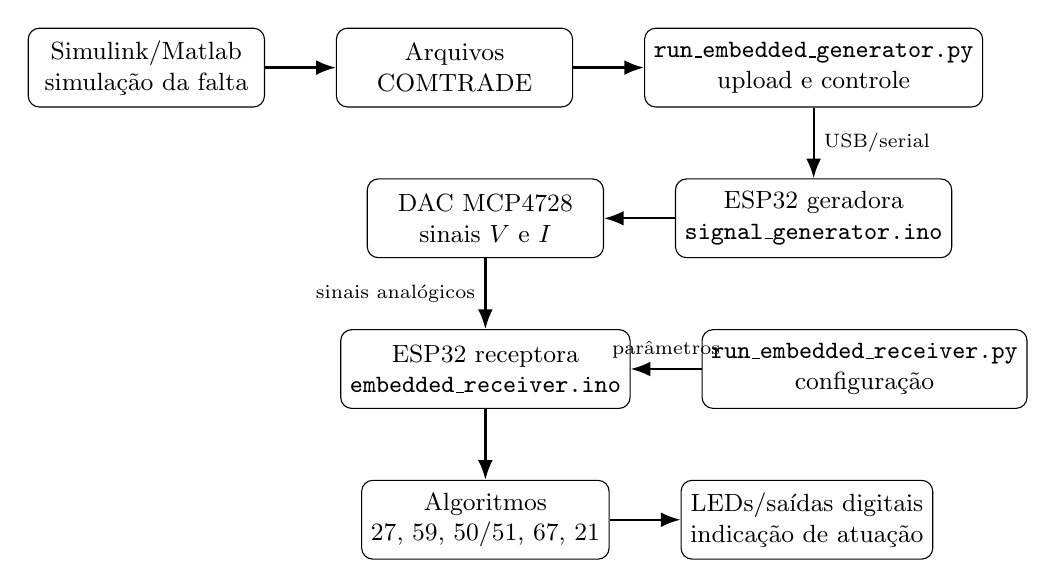
\begin{tikzpicture}[
    node distance=0.9cm,
    bloco/.style={draw, rounded corners, align=center, minimum width=3.0cm, minimum height=1.0cm, font=\small},
    seta/.style={-{Latex[length=2.5mm]}, thick}
  ]
    \node[bloco] (simulink) {Simulink/Matlab\\simulação da falta};
    \node[bloco, right=of simulink] (comtrade) {Arquivos\\COMTRADE};
    \node[bloco, right=of comtrade] (pcgen) {\texttt{run\_embedded\_generator.py}\\upload e controle};
    \node[bloco, below=of pcgen] (espgen) {ESP32 geradora\\\texttt{signal\_generator.ino}};
    \node[bloco, left=of espgen] (dac) {DAC MCP4728\\sinais $V$ e $I$};
    \node[bloco, below=of dac] (esprx) {ESP32 receptora\\\texttt{embedded\_receiver.ino}};
    \node[bloco, right=of esprx] (pcrx) {\texttt{run\_embedded\_receiver.py}\\configuração};
    \node[bloco, below=of esprx] (prot) {Algoritmos\\27, 59, 50/51, 67, 21};
    \node[bloco, right=of prot] (leds) {LEDs/saídas digitais\\indicação de atuação};

    \draw[seta] (simulink) -- (comtrade);
    \draw[seta] (comtrade) -- (pcgen);
    \draw[seta] (pcgen) -- node[right]{\scriptsize USB/serial} (espgen);
    \draw[seta] (espgen) -- (dac);
    \draw[seta] (dac) -- node[left]{\scriptsize sinais analógicos} (esprx);
    \draw[seta] (pcrx) -- node[above]{\scriptsize parâmetros} (esprx);
    \draw[seta] (esprx) -- (prot);
    \draw[seta] (prot) -- (leds);
  \end{tikzpicture}
  \caption{Arquitetura metodológica da plataforma proposta}
  \label{fig:arquitetura-metodologia}
\end{figure}

O fluxo metodológico foi dividido nas seguintes etapas:

\begin{itemize}
  \item modelagem e simulação da falta no Simulink;
  \item exportação das amostras de tensão e corrente para o Matlab;
  \item conversão das amostras para arquivos COMTRADE;
  \item validação e envio dos arquivos à ESP32 geradora;
  \item processamento local do registro na ESP32 geradora;
  \item reprodução analógica dos canais de tensão e corrente pelo DAC MCP4728;
  \item aquisição dos sinais pela ESP32 receptora;
  \item configuração dos parâmetros das funções de proteção;
  \item processamento fasorial das amostras recebidas;
  \item execução dos algoritmos de proteção;
  \item indicação da atuação por eventos seriais e por LEDs/saídas digitais.
\end{itemize}

\section{Geração das amostras no Simulink/Matlab}

A primeira etapa consiste na simulação de um sistema elétrico de potência no ambiente Simulink/Matlab. O modelo elétrico utilizado representa um sistema de transmissão em \SI{500}{\kilo\volt}, composto por fontes equivalentes, transformadores trifásicos, linha de transmissão, blocos de medição de tensão e corrente e bloco de aplicação de falta. A finalidade dessa etapa é gerar, de forma controlada, os sinais de tensão e corrente necessários para testar as funções de proteção implementadas na plataforma.

O modelo simulado é apresentado na Figura \ref{fig:modelo-simulink}. Nele, a fonte trifásica G1 alimenta o sistema por meio do transformador T1. Em seguida, os sinais passam pelo medidor trifásico de entrada, pelos trechos de linha de transmissão LT1-1 e LT1-2 e pelo medidor de saída antes de alcançar o transformador T2 e a fonte equivalente G2. O ponto de aplicação da falta trifásica é conectado ao barramento intermediário da linha, permitindo a obtenção das grandezas de curto-circuito no ponto de falta.

\begin{figure}[H]
  \centering
  \caption{Modelo de simulação do sistema elétrico no Simulink}
  \label{fig:modelo-simulink}

  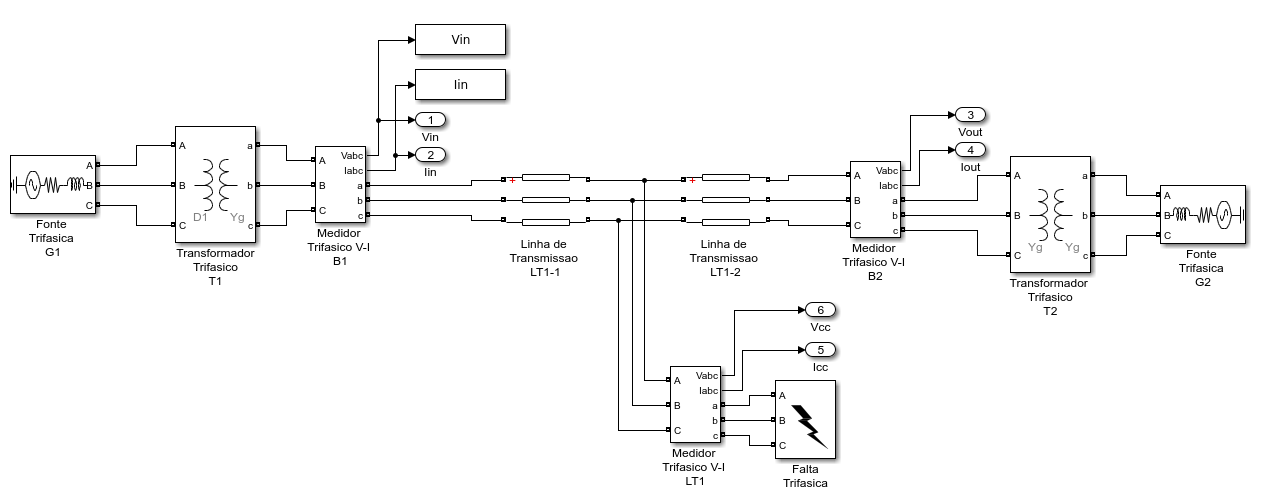
\includegraphics[width=\textwidth]{figuras/modelo_simulink.png}

  \legend{Fonte: Autoria própria.}
\end{figure}

Todos os testes descritos neste trabalho foram realizados considerando a condição de carregamento de 1 SIL, isto é, a potência natural da linha utilizada como referência operacional do sistema. Essa condição foi adotada para estabelecer um ponto nominal comum entre os ensaios, permitindo que as alterações realizadas para validar cada função de proteção fossem controladas em torno de uma mesma base de operação.

Os parâmetros elétricos da linha de transmissão utilizada no modelo são apresentados na Tabela \ref{tab:parametros-linha}. A linha possui tensão nominal de \SI{500}{\kilo\volt} e comprimento de \SI{190}{\kilo\metre}, sendo representada por parâmetros de sequência homopolar e não homopolar.

\begin{table}[H]
  \centering
  \small
  \caption{Parâmetros elétricos da linha de transmissão de \SI{500}{\kilo\volt} e \SI{190}{\kilo\metre}}
  \label{tab:parametros-linha}
  \begin{tabular}{lccc}
    \toprule
    Componente & Resistência & Reatância indutiva & Susceptância \\
    \midrule
    Homopolar & \SI{0,4352}{\ohm\per\kilo\metre} & \SI{1,4427}{\ohm\per\kilo\metre} & \SI{3,5227}{\micro\siemens\per\kilo\metre} \\
    Não homopolar & \SI{0,0161}{\ohm\per\kilo\metre} & \SI{0,2739}{\ohm\per\kilo\metre} & \SI{6,0417}{\micro\siemens\per\kilo\metre} \\
    \bottomrule
  \end{tabular}
  \legend{Fonte: Sistema teste utilizado nas simulações.}
\end{table}

Os dados do gerador equivalente utilizado na condição de 1 SIL são apresentados na Tabela \ref{tab:parametros-gerador}. Esses parâmetros definem a potência de referência, a tensão interna e a impedância associada à fonte do sistema.

\begin{table}[H]
  \centering
  \small
  \caption{Parâmetros do gerador equivalente para a condição de 1 SIL}
  \label{tab:parametros-gerador}
  \begin{tabular}{lcccc}
    \toprule
    Equipamento & Potência & Tensão & Reatância & Resistência \\
    \midrule
    Gerador G1 & \SI{1417,5}{\mega\volt\ampere} & $\SI{15,37}{\kilo\volt}\angle \ang{3,41}$ & \SI{0,04317}{\ohm} & \SI{0,001257}{\ohm} \\
    \bottomrule
  \end{tabular}
  \legend{Fonte: Sistema teste utilizado nas simulações.}
\end{table}

A Tabela \ref{tab:parametros-fonte-equivalente} apresenta os parâmetros da fonte equivalente associada ao terminal remoto do sistema. Foram considerados os parâmetros de 1 SIL, incluindo os valores de tensão e impedâncias equivalentes de Thévenin.

\begin{table}[H]
  \centering
  \small
  \caption{Parâmetros da fonte equivalente para a condição de 1 SIL}
  \label{tab:parametros-fonte-equivalente}
  \begin{tabular}{lccccc}
    \toprule
    Equipamento & Tensão & $R_{1vth}$ & $X_{1vth}$ & $R_{0vth}$ & $X_{0vth}$ \\
    \midrule
    Vth fraca & $\SI{501,27}{\kilo\volt}\angle \ang{-15,97}$ & \SI{7,6980}{\ohm} & \SI{46,188}{\ohm} & \SI{46,188}{\ohm} & \SI{230,9401}{\ohm} \\
    Vth forte & $\SI{498,70}{\kilo\volt}\angle \ang{-6,51}$ & \SI{1,9245}{\ohm} & \SI{11,5475}{\ohm} & \SI{11,5475}{\ohm} & \SI{57,7349}{\ohm} \\
    \bottomrule
  \end{tabular}
  \legend{Fonte: Sistema teste utilizado nas simulações.}
\end{table}

Os transformadores T1 e T2 foram modelados com enrolamentos em conexão $\Delta$/$Y_g$ e $Y_g$/$Y_g$, respectivamente. Os parâmetros elétricos utilizados na representação dos transformadores são apresentados na Tabela \ref{tab:parametros-transformador}.

\begin{table}[H]
  \centering
  \small
  \caption{Parâmetros dos transformadores utilizados no modelo}
  \label{tab:parametros-transformador}
  \begin{tabular}{lc}
    \toprule
    Parâmetro & Valor \\
    \midrule
    Reatância de dispersão do primário (\SI{15}{\kilo\volt}) & \SI{0,0846}{\ohm} \\
    Reatância de dispersão do secundário (\SI{525}{\kilo\volt}) & \SI{31,3380}{\ohm} \\
    Resistência do enrolamento do primário (\SI{15}{\kilo\volt}) & \SI{0,0030}{\ohm} \\
    Resistência do enrolamento do secundário (\SI{525}{\kilo\volt}) & \SI{0,7950}{\ohm} \\
    \bottomrule
  \end{tabular}
  \legend{Fonte: Sistema teste utilizado nas simulações.}
\end{table}

Durante a simulação, são definidos o instante de aplicação da falta, a duração do evento, a frequência nominal, a taxa de amostragem e os canais medidos. As amostras geradas pelo Simulink são enviadas ao workspace do Matlab. A partir desse ponto, os vetores de tempo, tensão e corrente passam a compor a base de dados que será convertida para oscilografia. Essa etapa é importante porque preserva a relação temporal entre os sinais, permitindo que a reprodução física posterior mantenha coerência com o evento simulado.

\begin{figure}[H]
  \centering
  \caption{Amostras simuladas de tensão e corrente}
  \label{fig:amostras-simulink}

  \fbox{\parbox{0.85\textwidth}{\centering Espaço reservado para gráfico das formas de onda simuladas de tensão e corrente antes, durante e após a falta.}}

  \legend{Fonte: Autoria própria.}
\end{figure}

\subsection{Cenários de validação das funções de proteção}

As simulações não foram utilizadas apenas para gerar uma única condição de curto-circuito, mas para construir cenários específicos de validação para cada função de proteção. Dessa forma, os parâmetros do sistema foram alterados de maneira controlada para produzir condições compatíveis com os ajustes definidos no relé emulado.

Para a validação das funções de subtensão e sobretensão, a saída do transformador T1 foi ajustada propositalmente para que a tensão medida no ponto de interesse ficasse abaixo ou acima dos limites configurados na proteção. Assim, foi possível verificar se a função ANSI 27 atuava quando a tensão permanecia inferior ao valor de pickup e se a função ANSI 59 atuava quando a tensão ultrapassava o limite superior configurado.

Para a validação da função de sobrecorrente, a relação de impedância entre os trechos LT1-1 e LT1-2 foi alterada de forma a modificar a corrente observada durante a falta. Ao reduzir ou aumentar a impedância equivalente vista pelo ponto de falta, a corrente de curto-circuito também se altera, permitindo testar diferentes valores de pickup das funções ANSI 50 e ANSI 51.

Para a validação da função de distância, foram simuladas condições nas quais a impedância aparente vista pelo ponto de medição permanecesse dentro ou fora das zonas configuradas. Essa avaliação é feita a partir da relação entre os fasores de tensão e corrente medidos, permitindo verificar a atuação das zonas da função ANSI 21 de acordo com o alcance configurado para a linha.

Por fim, para a função direcional, a validação foi realizada por meio da alteração do ângulo entre as fontes G1 e G2. Essa alteração modifica o sentido do fluxo de potência no sistema, permitindo criar condições de fluxo direto ou reverso. Dessa forma, a função ANSI 67 pôde ser avaliada quanto à capacidade de permitir ou bloquear a atuação da proteção conforme a direção estimada da falta.

A estratégia de ensaio adotada para cada proteção é resumida na Tabela \ref{tab:cenarios-protecao}.

\begin{table}[H]
  \centering
  \small
  \caption{Cenários simulados para validação das funções de proteção}
  \label{tab:cenarios-protecao}
  \begin{tabular}{lll}
    \toprule
    Função & Parâmetro alterado na simulação & Objetivo do ensaio \\
    \midrule
    27 & Tensão na saída de T1 & Produzir tensão abaixo do pickup \\
    59 & Tensão na saída de T1 & Produzir tensão acima do pickup \\
    50/51 & Impedância entre LT1-1 e LT1-2 & Variar corrente de curto-circuito \\
    21 & Impedância aparente vista pelo relé & Testar atuação por zonas \\
    67 & Ângulo entre G1 e G2 & Alterar sentido do fluxo de potência \\
    \bottomrule
  \end{tabular}
  \legend{Fonte: Autoria própria.}
\end{table}

\section{Conversão das amostras para COMTRADE}

Após a simulação, as amostras são processadas pelo script \texttt{comtrade\_generator.m}. Esse script organiza os dados provenientes do Matlab e gera os arquivos do registro COMTRADE, principalmente o arquivo de configuração \texttt{.cfg} e o arquivo de dados correspondente.

O arquivo \texttt{.cfg} contém informações necessárias para interpretação do registro, como identificação do ensaio, frequência nominal, taxa de amostragem, número de canais, unidades e fatores de escala. O arquivo de dados contém os valores amostrados ao longo do tempo. Esse formato é importante porque aproxima o projeto de uma prática real de análise de faltas, visto que o COMTRADE é amplamente utilizado em estudos de oscilografias e eventos em sistemas elétricos de potência \cite{ieee_comtrade,iec_60255_24_2013}.

Do ponto de vista metodológico, essa etapa transforma uma simulação computacional em um registro padronizado. Assim, a plataforma deixa de depender apenas do ambiente Simulink e passa a operar a partir de um formato que pode ser reaproveitado, validado e futuramente substituído por registros de outras origens.

\begin{figure}[H]
  \centering
  \fbox{\parbox{0.85\textwidth}{\centering Espaço reservado para imagem ou captura dos arquivos COMTRADE gerados, destacando os arquivos \texttt{.cfg} e \texttt{.dat}/\texttt{.bdat}.}}
  \caption{Arquivos COMTRADE gerados a partir das amostras simuladas}
  \label{fig:arquivos-comtrade}
\end{figure}

\section{Validação e preparação dos arquivos}

Antes de enviar os arquivos à ESP32 geradora, é necessário verificar se o registro é compatível com a plataforma. Essa validação busca evitar que arquivos incompletos, com canais incompatíveis ou taxas de amostragem inadequadas sejam utilizados nos ensaios.

Os principais critérios considerados são:

\begin{itemize}
  \item existência dos arquivos de configuração e dados;
  \item presença dos canais analógicos necessários;
  \item identificação de um canal de tensão e um canal de corrente;
  \item taxa de amostragem compatível com a reprodução;
  \item quantidade de amostras compatível com a memória disponível;
  \item formato dos dados aceito pela versão embarcada do gerador.
\end{itemize}

Na versão atual do projeto, o script \texttt{run\_embedded\_generator.py} atua como interface de upload e controle da ESP32 geradora. Diferentemente das primeiras versões, nas quais o computador realizava maior parte do tratamento das amostras, a versão atual transfere o processamento principal para a ESP32. Assim, o computador envia os arquivos e a placa realiza localmente a interpretação, escala e preparação dos quadros de reprodução.

\begin{figure}[H]
  \centering
  \fbox{\parbox{0.85\textwidth}{\centering Espaço reservado para captura da etapa de validação/preparação dos arquivos ou tela do terminal antes do envio à ESP32 geradora.}}
  \caption{Validação e preparação dos arquivos para reprodução}
  \label{fig:validacao-arquivos}
\end{figure}

\section{Envio dos dados para a ESP32 geradora}

O envio dos arquivos ocorre por comunicação USB/serial. O script \texttt{run\_embedded\_generator.py} abre a porta serial da ESP32 geradora, aguarda a mensagem de prontidão da placa, envia o arquivo \texttt{.cfg} e o arquivo de dados em blocos e verifica as confirmações de recebimento.

Após o upload, o script solicita o processamento local do registro. A ESP32 geradora interpreta o arquivo de configuração, identifica os canais, calcula os parâmetros de escala e organiza as amostras em estruturas internas de reprodução. Ao final desse processamento, a placa informa que está pronta para reproduzir o evento.

Além disso, o processo gera um arquivo de configuração auxiliar para a ESP32 receptora. Esse arquivo contém informações como escala dos canais, frequência de referência, taxa de amostragem recomendada, valores nominais e mapeamento dos canais de aquisição. Essa etapa é importante para que a recepção interprete corretamente os sinais reproduzidos pela unidade geradora.

\begin{figure}[H]
  \centering
  \fbox{\parbox{0.85\textwidth}{\centering Espaço reservado para captura do terminal durante o upload dos arquivos e confirmação \texttt{READY\_PLAYBACK} da ESP32 geradora.}}
  \caption{Envio dos arquivos COMTRADE para a ESP32 geradora}
  \label{fig:upload-esp32-geradora}
\end{figure}

\section{Reprodução dos sinais na ESP32 geradora}

A ESP32 geradora utiliza o firmware \path{embedded_generator.ino}. Esse firmware é responsável por armazenar os arquivos recebidos, processar o COMTRADE, construir os quadros de reprodução e comandar o DAC MCP4728. O conversor digital-analógico possui resolução de 12 bits e quatro canais, sendo utilizado para reproduzir os sinais de tensão e corrente em forma analógica \cite{microchip_mcp4728}.

Como o DAC trabalha em uma faixa positiva de tensão, os sinais alternados são reproduzidos com um deslocamento em torno de uma tensão média. Dessa forma, uma senoide que originalmente teria valores positivos e negativos é mapeada para uma faixa compatível com o hardware. A Figura \ref{fig:geracao-sinais} ilustra a lógica de reprodução.

\begin{figure}[H]
  \centering
  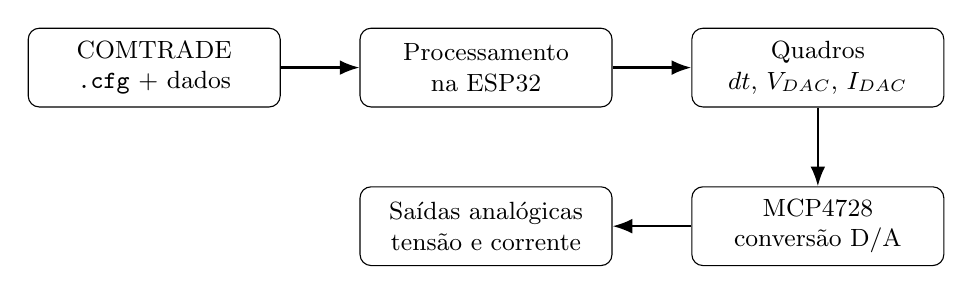
\begin{tikzpicture}[
    node distance=1.0cm,
    bloco/.style={draw, rounded corners, align=center, minimum width=3.2cm, minimum height=1.0cm, font=\small},
    seta/.style={-{Latex[length=2.5mm]}, thick}
  ]
    \node[bloco] (cfg) {COMTRADE\\\texttt{.cfg} + dados};
    \node[bloco, right=of cfg] (proc) {Processamento\\na ESP32};
    \node[bloco, right=of proc] (frames) {Quadros\\$dt$, $V_{DAC}$, $I_{DAC}$};
    \node[bloco, below=of frames] (dac) {MCP4728\\conversão D/A};
    \node[bloco, left=of dac] (out) {Saídas analógicas\\tensão e corrente};

    \draw[seta] (cfg) -- (proc);
    \draw[seta] (proc) -- (frames);
    \draw[seta] (frames) -- (dac);
    \draw[seta] (dac) -- (out);
  \end{tikzpicture}
  \caption{Etapas de preparação e reprodução dos sinais na ESP32 geradora}
  \label{fig:geracao-sinais}
\end{figure}

O firmware permite diferentes modos de reprodução. O modo de teste gera uma senoide para verificação da bancada. O modo de pré-falta reproduz continuamente os ciclos anteriores ao evento, permitindo estabilizar a recepção antes da falta. O modo de reprodução completa executa o registro COMTRADE, incluindo o período pré-falta, o instante da falta e o comportamento posterior. Esses modos tornam o ensaio repetível e facilitam a visualização do comportamento da proteção.

\begin{figure}[H]
  \centering
  \fbox{\parbox{0.85\textwidth}{\centering Espaço reservado para foto da ESP32 geradora conectada ao DAC MCP4728.}}
  \caption{Unidade embarcada de geração dos sinais}
  \label{fig:unidade-geradora}
\end{figure}

\begin{figure}[H]
  \centering
  \fbox{\parbox{0.85\textwidth}{\centering Espaço reservado para imagem do sinal analógico reproduzido, obtida por osciloscópio, captura ADC ou gráfico de validação.}}
  \caption{Sinais analógicos de tensão e corrente reproduzidos pelo DAC}
  \label{fig:sinais-reproduzidos}
\end{figure}

\section{Aquisição dos sinais na ESP32 receptora}

Os sinais analógicos reproduzidos pelo DAC são aplicados às entradas analógicas da ESP32 receptora. Essa unidade utiliza o firmware \path{embedded_receiver.ino}, responsável por realizar a aquisição dos canais de tensão e corrente, remover o nível médio dos sinais, aplicar os fatores de escala e organizar as amostras para processamento.

A recepção é configurada por meio do script \texttt{run\_embedded\_receiver.py}. Esse script envia à ESP32 receptora os parâmetros necessários para o ensaio, incluindo taxa de amostragem, escalas, valores nominais, frequência de referência e ajustes das funções de proteção. Depois da configuração, a aquisição e a análise são executadas de forma embarcada.

A Figura \ref{fig:recepcao-protecao} apresenta a sequência funcional da unidade receptora.

\begin{figure}[H]
  \centering
  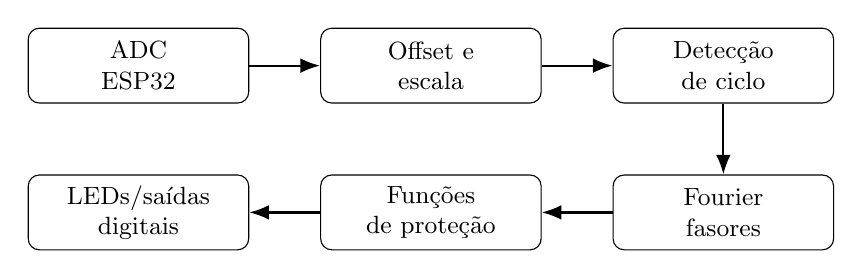
\begin{tikzpicture}[
    node distance=0.9cm,
    bloco/.style={draw, rounded corners, align=center, minimum width=2.8cm, minimum height=0.95cm, font=\small},
    seta/.style={-{Latex[length=2.5mm]}, thick}
  ]
    \node[bloco] (adc) {ADC\\ESP32};
    \node[bloco, right=of adc] (escala) {Offset e\\escala};
    \node[bloco, right=of escala] (ciclo) {Detecção\\de ciclo};
    \node[bloco, below=of ciclo] (fourier) {Fourier\\fasores};
    \node[bloco, left=of fourier] (reles) {Funções\\de proteção};
    \node[bloco, left=of reles] (leds) {LEDs/saídas\\digitais};

    \draw[seta] (adc) -- (escala);
    \draw[seta] (escala) -- (ciclo);
    \draw[seta] (ciclo) -- (fourier);
    \draw[seta] (fourier) -- (reles);
    \draw[seta] (reles) -- (leds);
  \end{tikzpicture}
  \caption{Fluxo de aquisição, processamento e atuação na ESP32 receptora}
  \label{fig:recepcao-protecao}
\end{figure}

\begin{figure}[H]
  \centering
  \fbox{\parbox{0.85\textwidth}{\centering Espaço reservado para foto da ESP32 receptora conectada aos canais analógicos e aos indicadores de atuação.}}
  \caption{Unidade embarcada de recepção e proteção}
  \label{fig:unidade-receptora}
\end{figure}

\section{Processamento das amostras recebidas}

Após a aquisição, as amostras são convertidas para grandezas de engenharia. Como os sinais reproduzidos pelo DAC são deslocados para uma faixa positiva de tensão, a primeira etapa consiste em estimar e remover o offset. Em seguida, aplica-se a escala calculada a partir do registro COMTRADE para recuperar a correspondência entre o sinal de bancada e a grandeza elétrica simulada.

O firmware organiza as amostras por ciclos elétricos. A cada ciclo, são estimadas grandezas como tensão fundamental, corrente fundamental, magnitude dos fasores, ângulo entre tensão e corrente, frequência estimada e indicadores de qualidade da aquisição. A Transformada de Fourier é utilizada porque permite obter magnitude e fase da componente fundamental, informações necessárias para funções como direcional e distância.

Esse processamento cria a ponte entre a forma de onda recebida e a decisão de proteção. Em outras palavras, a ESP32 receptora deixa de trabalhar apenas com valores instantâneos de ADC e passa a operar com grandezas elétricas equivalentes às utilizadas por relés digitais.

\begin{figure}[H]
  \centering
  \fbox{\parbox{0.85\textwidth}{\centering Espaço reservado para gráfico ou captura das grandezas processadas: tensão fundamental, corrente fundamental, fasores, impedância aparente ou eventos calculados.}}
  \caption{Processamento das amostras adquiridas pela ESP32 receptora}
  \label{fig:processamento-receptor}
\end{figure}

\section{Configuração das funções de proteção}

As funções de proteção são configuradas antes do início da aquisição. Essa configuração é realizada por comandos enviados pelo script \texttt{run\_embedded\_receiver.py}, permitindo habilitar ou desabilitar funções e definir os parâmetros de atuação. Essa característica aproxima a plataforma da lógica de ajuste de um relé real.

As principais funções previstas na plataforma são:

\begin{itemize}
  \item subtensão, função ANSI 27, ajustada por percentual de tensão e tempo de atuação;
  \item sobretensão, função ANSI 59, ajustada por percentual de tensão e tempo de atuação;
  \item sobrecorrente instantânea e temporizada, funções ANSI 50 e 51, ajustadas por pickup e atraso;
  \item direcional de sobrecorrente, função ANSI 67, ajustada por sentido, ângulo e janela angular;
  \item distância, função ANSI 21, ajustada por impedância da linha, alcance das zonas e temporização.
\end{itemize}

No caso de falta trifásica, a análise das funções de sobrecorrente e distância torna-se especialmente relevante. A sobrecorrente responde à elevação da corrente durante a falta, enquanto a distância avalia a impedância aparente calculada pela relação entre os fasores de tensão e corrente. A função direcional pode ser associada à função de distância para permitir ou bloquear a atuação, demonstrando a interação entre funções de proteção.

\begin{figure}[H]
  \centering
  \fbox{\parbox{0.85\textwidth}{\centering Espaço reservado para captura do terminal com os comandos de configuração das funções de proteção.}}
  \caption{Configuração das funções de proteção por comandos}
  \label{fig:configuracao-protecoes}
\end{figure}

\section{Lógica de atuação e indicação por LEDs}

A atuação das proteções ocorre quando as grandezas calculadas satisfazem os critérios configurados. Para proteções temporizadas, além da condição elétrica, é necessário que o tempo ajustado seja cumprido. Quando uma função atua, a ESP32 receptora registra o evento e mantém o estado de trip até que seja enviado um comando de reset ou que a placa seja reiniciada.

No projeto, a indicação da atuação é feita por mensagens seriais e por saídas digitais conectadas a LEDs ou a um módulo de relés. A versão atual da ESP32 receptora disponibiliza quatro indicações principais associadas à lógica de distância e direcional:

\begin{itemize}
  \item bloqueio da atuação da função de distância pela lógica direcional;
  \item permissão ou habilitação da atuação;
  \item trip da zona 1 da proteção de distância;
  \item trip da zona 2 da proteção de distância.
\end{itemize}

Esses indicadores permitem visualizar fisicamente o resultado dos algoritmos de proteção. Assim, ao reproduzir uma oscilografia de falta, o aluno pode observar não apenas a forma de onda, mas também o comportamento lógico do relé emulado: condição normal, pickup, bloqueio, permissão e trip.

\begin{figure}[H]
  \centering
  \fbox{\parbox{0.85\textwidth}{\centering Espaço reservado para foto dos LEDs ou módulo de relés indicando bloqueio, permissão, zona 1 e zona 2.}}
  \caption{Indicação física da atuação das proteções}
  \label{fig:indicacao-leds}
\end{figure}

\section{Procedimento experimental}

O procedimento experimental segue uma sequência padronizada para garantir repetibilidade dos ensaios. Inicialmente, seleciona-se a oscilografia COMTRADE correspondente à falta a ser analisada. Em seguida, o script \texttt{run\_embedded\_generator.py} envia os arquivos à ESP32 geradora e solicita o processamento local. Após a confirmação de prontidão, a unidade geradora permanece disponível para executar os modos de teste, pré-falta ou reprodução completa.

Na sequência, a ESP32 receptora é configurada por meio do script \texttt{run\_embedded\_receiver.py}. São definidos os parâmetros de escala e os ajustes das funções de proteção que serão avaliadas no ensaio. Após a configuração, inicia-se a aquisição embarcada.

Com a recepção em execução, a ESP32 geradora reproduz os sinais analógicos de tensão e corrente. Esses sinais são recebidos pela ESP32 receptora, processados por ciclo e avaliados pelos algoritmos de proteção. Durante o ensaio, observam-se os eventos enviados pela serial e os LEDs/saídas digitais correspondentes à atuação das funções.

\begin{figure}[H]
  \centering
  \fbox{\parbox{0.85\textwidth}{\centering Espaço reservado para foto geral da bancada experimental com computador, ESP32 geradora, DAC, ESP32 receptora e LEDs.}}
  \caption{Bancada experimental utilizada nos ensaios}
  \label{fig:bancada-experimental}
\end{figure}

\section{Critérios de avaliação}

A avaliação da plataforma considera critérios funcionais e didáticos. Do ponto de vista funcional, verifica-se se a oscilografia é corretamente convertida, se o COMTRADE é aceito pela plataforma, se a ESP32 geradora reproduz os sinais, se a ESP32 receptora consegue adquirir as amostras e se as funções de proteção atuam de acordo com os parâmetros configurados.

Do ponto de vista didático, avalia-se se o sistema permite acompanhar todo o encadeamento do estudo de proteção: simulação da falta, geração da oscilografia, reprodução física, aquisição, processamento fasorial, decisão do relé e indicação por LEDs. Esse encadeamento é a principal contribuição metodológica da plataforma, pois transforma um conteúdo usualmente teórico em uma experiência prática e observável.

\section{Conclusão}

Este capítulo apresentou a metodologia utilizada no desenvolvimento da plataforma didática. Foram descritas as etapas de simulação, geração de arquivos COMTRADE, validação, envio à ESP32 geradora, reprodução dos sinais pelo DAC MCP4728, aquisição pela ESP32 receptora, processamento fasorial, configuração das funções de proteção e indicação da atuação por LEDs ou saídas digitais.

A metodologia proposta permite integrar ferramentas computacionais e hardware embarcado em um fluxo experimental único. Essa integração possibilita que eventos simulados em sistemas elétricos de potência sejam reproduzidos em bancada e analisados por algoritmos de proteção, estabelecendo a base para a implementação detalhada apresentada no capítulo seguinte.

\chapter{Implementação}

\section{Hardware Utilizado}

O hardware da plataforma é composto por duas placas ESP32, um conversor digital-analógico MCP4728, conexões USB para comunicação serial e canais analógicos destinados à reprodução e recepção dos sinais de tensão e corrente.

\begin{table}[H]
  \centering
  \caption{Principais componentes da plataforma}
  \label{tab:componentes}
  \begin{tabular}{ll}
    \toprule
    Componente & Função \\
    \midrule
    ESP32 geradora & Receber amostras e controlar a reprodução dos sinais \\
    MCP4728 & Converter amostras digitais em sinais analógicos \\
    ESP32 receptora & Adquirir sinais analógicos e executar algoritmos de proteção \\
    Computador & Configuração, envio de arquivos e supervisão dos testes \\
    \bottomrule
  \end{tabular}
\end{table}

\section{Software Desenvolvido}

O desenvolvimento do projeto é organizado em scripts e firmwares específicos:

\begin{itemize}
  \item \texttt{comtrade\_generator.m}: gera os arquivos COMTRADE a partir das amostras do Simulink.
  \item \path{run_embedded_generator.py}: valida, interpreta e envia as amostras COMTRADE à ESP32 geradora.
  \item \path{embedded_generator.ino}: firmware responsável pela recepção, bufferização e reprodução dos sinais.
  \item \texttt{run\_embedded\_receiver.py}: executa a interface de controle e supervisão da ESP32 receptora.
  \item \path{embedded_receiver.ino}: firmware responsável pela aquisição das amostras e execução dos algoritmos de proteção.
\end{itemize}

\section{Protocolo de Comunicação}

A comunicação entre o computador e as ESP32 ocorre por interface USB/serial. As amostras são empacotadas em mensagens contendo informações de amplitude, canal e controle de execução. O protocolo deve permitir identificar o início e o fim da transmissão, a separação entre canais de tensão e corrente e a confirmação de recebimento dos blocos de dados.

\section{Bufferização e Reprodução}

A bufferização das amostras é necessária para reduzir falhas de temporização durante a reprodução. O firmware da ESP32 geradora organiza as amostras recebidas em memória e atualiza os canais do DAC conforme a taxa de amostragem definida pelo arquivo COMTRADE. Dessa forma, busca-se preservar a forma de onda original dentro das limitações de resolução, velocidade e faixa de tensão do hardware utilizado.

\section{Aquisição e Processamento}

Na unidade receptora, os sinais analógicos são convertidos em amostras digitais. Em seguida, janelas de amostras são processadas para estimativa das grandezas utilizadas nos algoritmos de proteção. A Transformada de Fourier é aplicada para extração da componente fundamental, permitindo obter magnitude e fase dos sinais de tensão e corrente.

\section{Algoritmos de Proteção}

Os algoritmos de proteção foram estruturados para permitir operação individual ou combinada das funções implementadas. Cada função possui parâmetros próprios de ajuste, configurados de forma semelhante ao processo adotado em relés reais. Essa característica possibilita estudar a influência dos ajustes sobre a atuação do sistema.

Além disso, a arquitetura permite a interação entre funções de proteção. Por exemplo, uma lógica direcional pode ser utilizada em conjunto com uma função de distância, permitindo avaliar estratégias de proteção mais próximas das empregadas em sistemas elétricos reais.

\chapter{Resultados e Discussão}

\section{Integração funcional da plataforma}

% Seção reservada para os resultados definidos pelo autor.

\section{Reprodução, aquisição e observabilidade}

% Seção reservada para os resultados definidos pelo autor.

\section{Resposta das funções de proteção}

% Seção reservada para os resultados definidos pelo autor.

\section{Aplicabilidade didática}

% Seção reservada para os resultados definidos pelo autor.

\section{Discussão das limitações}

% Seção reservada para os resultados definidos pelo autor.

\chapter{Considerações Finais}

Este trabalho apresentou o desenvolvimento de uma plataforma didática embarcada para reprodução de registros COMTRADE e emulação de funções de proteção de sistemas elétricos de potência. A solução utiliza duas placas ESP32: a unidade geradora interpreta um registro binário, forma quadros temporizados e reproduz um canal de tensão e um de corrente pelo MCP4728; a unidade receptora adquire esses sinais, estima os fasores fundamentais e avalia as funções ANSI 21, 27, 50, 51, 59 e 67.

A arquitetura alcançada mantém nas ESP32 o caminho de tempo crítico e utiliza o computador para simulação, transferência, configuração e supervisão. O \texttt{config.json} vincula cada COMTRADE às escalas e referências empregadas na recepção, reduzindo ambiguidades entre os domínios elétrico, digital e analógico. Os protocolos de confirmação, os indicadores de qualidade, os eventos seriais e as saídas físicas tornam observável o percurso entre a oscilografia e a decisão de proteção.

Do ponto de vista didático, a plataforma aproxima conceitos de COMTRADE, amostragem, DFT, impedância aparente, pickup, temporização e supervisão direcional de uma experiência reconfigurável em bancada. Sua contribuição principal é a integração funcional e rastreável desses elementos em hardware de baixo custo. O protótipo não substitui uma mala de testes, um relé comercial ou um sistema calibrado, pois não dispõe de condicionamento e isolamento próprios nem foi submetido a uma caracterização metrológica completa.

A observação experimental estabeleceu \SI{1000}{amostras\per\second} como limite operacional para a reprodução coerente dos sinais de \SI{60}{\hertz} avaliados. Acima dessa taxa, houve perda de sincronismo temporal. Esse comportamento, somado às restrições do buffer, da interpolação, do ADC interno e da montagem em protoboard, delimita a validade dos ensaios e evidencia a necessidade de verificar qualidade temporal, saturação e continuidade, e não apenas o estado final de trip.

Como trabalhos futuros, recomendam-se uma matriz quantitativa e repetível de testes para todas as funções implementadas; medição sincronizada dos erros de amplitude, fase e tempo; expansão para três tensões e três correntes; suporte direto a outros formatos e ordenações COMTRADE; condicionamento analógico e isolamento em placa dedicada; avaliação de ADCs externos; curvas inversas para a função 51; comparadores angulares adicionais para a função 67; e comparação experimental com relés comerciais. Essas extensões podem transformar o protótipo funcional em uma bancada didática mais abrangente e metrologicamente caracterizada.


\postextual

\bibliographystyle{abntex2-alf}
\bibliography{referencias}

\appendix
\chapter{Trechos de Código e Comandos de Execução}

Este apêndice deve reunir trechos representativos dos scripts e firmwares desenvolvidos, bem como exemplos de comandos utilizados durante os ensaios.

\section{Geração e Reprodução}

Inserir trechos relevantes dos arquivos \texttt{generate\_signal\_v6.py} e \texttt{v\_6.ino}, destacando a leitura dos arquivos COMTRADE, o envio das amostras, a bufferização e a atualização do DAC MCP4728.

\section{Recepção e Proteção}

Inserir trechos relevantes dos arquivos \texttt{run\_embedded\_receiver.py} e \texttt{v\_2.ino}, destacando a aquisição das amostras, o processamento pela Transformada de Fourier e a execução das funções de proteção.

\section{Exemplos de Comandos}

Inserir exemplos de comandos de execução utilizados para configurar e testar cada função de proteção.


\end{document}
